%# -*- coding: utf-8-unix -*-
% !TEX program = xelatex
% !TEX root = ../thesis.tex

\chapter{Conclusion}

\section{Thesis Contributions}

    This thesis attracts researchers' attention on programming education.
    We explained online judges in detail.
    Proactive students demands online judges to advise them which problems of the thousand ones to solve.
    We proposed to use reinforcement learning to design problem set for each student.
    To tackle the problem that the training process of reinforcement learning algorithms
    requires intensive interaction data,
    we introduced a user model to fit students' mindset with real-world submission history.
    We believe that this framework would be a general method to enable reinforcement learning in the education area.
    Experiment data show that our algorithm outperforms human teachers,
    based on metrics of our user model.

    We wish this work would have real-world impact and call on researchers to dive further into programming education.

\section{Future Work}

    During the development of this thesis, we encountered some problems that have not yet been solved.
    Future researchers might start further study by addressing these problems.

    The biggest question in our mind is the effectiveness and the interpretability of user models.
    We believe that a good user model should at least adhere to intuition.
    For example, we would expect that the overall skills of a user should generally increase
    as the user has solved more problem.
    In our recurrent neural network user model, we are not able to see this trend on all students
    (see Figure \ref{fig:user model interpretability}).

    \begin{figure}
        \centering
        \begin{subfigure}[b]{0.475\textwidth}
            \centering
            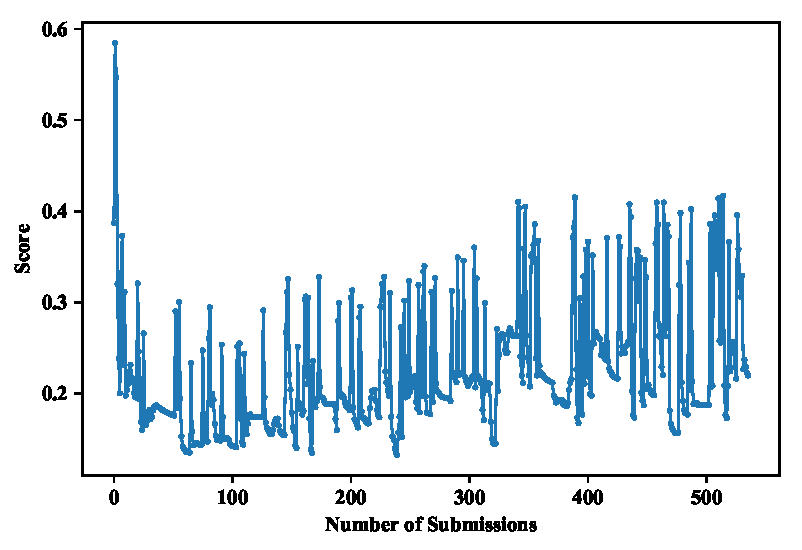
\includegraphics[width=\textwidth]{img/submit-score-user-1830.pdf}
        \end{subfigure}
        \hfill
        \begin{subfigure}[b]{0.475\textwidth}
            \centering
            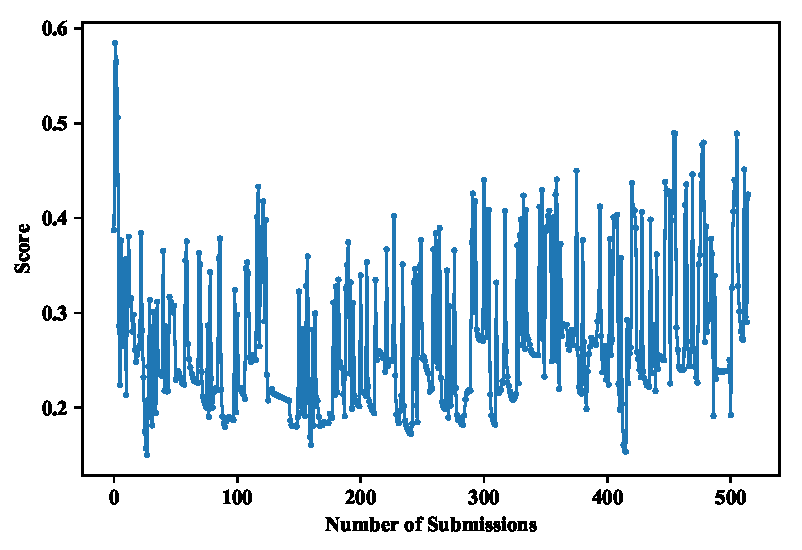
\includegraphics[width=\textwidth]{img/submit-score-user-1749.pdf}
        \end{subfigure}
        \vskip\baselineskip
        \begin{subfigure}[b]{0.475\textwidth}
            \centering
            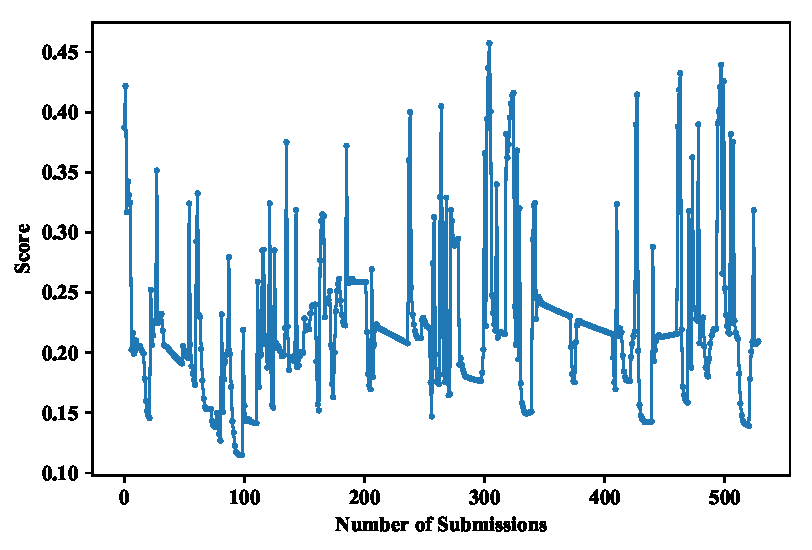
\includegraphics[width=\textwidth]{img/submit-score-user-1013.pdf}
        \end{subfigure}
        \hfill
        \begin{subfigure}[b]{0.475\textwidth}
            \centering
            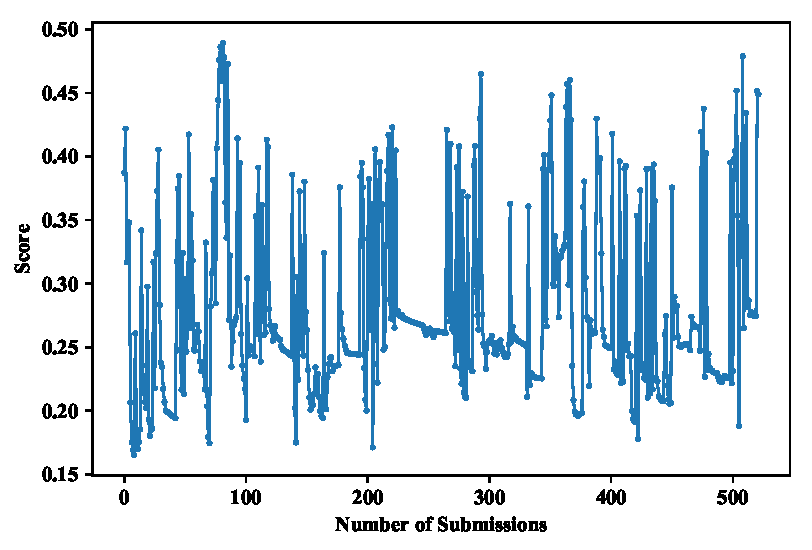
\includegraphics[width=\textwidth]{img/submit-score-user-2799.pdf}
        \end{subfigure}
        \caption[Plot of user score and the number of submissions]{
            Plot of user score and the number of submissions.
            The upper two figures shows the rising trend slightly if not at all.
            The lower two figures does not show any reasonable pattern.
        }
        \label{fig:user model interpretability}
    \end{figure}

    Another problem is how to measure the mastery of a student.
    Currently, we define ``user score'' as the average over all possibilities of the student able to solve a problem.
    We believe that more sophisticated metrics can be used.

    We also feel that the data used in this thesis is far from ideal.
    The data is clustered and highly biased.
    We expect our methods to have better results on a more typical data set.
    On the other hand, the data is from a real online judge.
    It puts another challenge on how to design optimal problem sets for students on online judges like this.





